\section{Consistencia causal y comparación de métodos}
\label{sec:auditoria-actual-resultados}

La pregunta que orienta la propuesta es si una selección estructurada de
semillas permite localizar, con un presupuesto declarado, candidatos que no
se encuentran al iniciar cerca de los equilibrios. Esta pregunta debe
distinguirse de otras dos: si los candidatos son atractores en un espacio de
estados adecuado y si su cuenca evita una vecindad completa de todos los
equilibrios. La primera admite un contraste computacional finito; las otras
requieren argumentos adicionales de existencia, atracción y separación.

La metodología combina realizaciones de Lur'e, aproximaciones armónicas,
puntos perpetuos y continuación. Para comparar estas rutas relacionamos
sus hipótesis con el destino calculado y el costo de integración. La
geometría del campo organiza la búsqueda, mientras que la atracción y la
posición de la cuenca se estudian sobre la respuesta alcanzada.

\subsection{Equilibrios, semillas y conjuntos atrayentes}

Consideramos cuatro objetos de naturaleza distinta. Un equilibrio es una
raíz exacta de $F(e)=0$. Una semilla es un dato que propone una búsqueda; su
origen puede ser una identidad algebraica o una aproximación armónica. Una
trayectoria calculada es una aproximación de un problema de valor inicial
especificado. Un atractor es un objeto invariante y atrayente respecto de un
espacio, una topología y una familia de datos iniciales. La relación entre ellos se establece resolviendo las ecuaciones y
analizando la evolución, no sólo mediante el residuo de una semilla.

En orden entero, el flujo local permite concatenar soluciones mientras
existan. Para Caputo con terminal inferior fijo, el dato puntual en un
instante intermedio no determina por sí solo la continuación: falta la
contribución de la historia anterior. El reinicio sobre constantes constituye
una sección de datos admisibles, no todo el espacio funcional. Por ello las
expresiones \emph{cuenca de reinicios}, \emph{atracción funcional} y
\emph{atracción uniforme de conjuntos acotados} deben conservar sus
definiciones distintas de las secciones anteriores.

\begin{longtable}{L{.21\linewidth}L{.35\linewidth}L{.35\linewidth}}
\caption{Pregunta, objeto y evidencia que puede responderla.}
\label{tab:revision-preguntas}\\
\toprule
Pregunta & Cálculo & Límite\\\midrule
\endfirsthead
\toprule Pregunta & Cálculo & Límite\\\midrule
\endhead
¿Es exacta la realización? & Sustituir matrices y no linealidad; verificar
identidad en el dominio declarado. & Una coincidencia puntual no comprueba
una identidad funcional.\\
¿Es admisible la semilla? & Residuo armónico, rama compleja, ganancia,
denominadores y reconstrucción del estado. & Residuo pequeño no implica una
órbita periódica causal.\\
¿Se calculó el mismo PVI? & Igual campo, parámetros, orden, terminal inferior,
historia y reglas de reinicio. & Estados finales parecidos no
identifican la historia.\\
¿Hay persistencia numérica? & Comparar pasos, horizontes y métodos bajo
escalas y tolerancias fijadas. & Acotación finita no prueba convergencia ni
acotación para todo tiempo.\\
¿Hay caos? & Diagnósticos complementarios con ventana, muestreo y memoria
declarados; controles negativos. & Una FFT o un exponente estimado aislado
no constituye una prueba.\\
¿Hay ocultación? & Separar una región próxima a cada equilibrio de la
cuenca del candidato; declarar el espacio de estados. & Cero contactos en
una muestra finita no excluye todos los puntos de una bola.\\
\bottomrule
\end{longtable}

\subsection{Un control analítico del efecto de reiniciar la memoria}

Considérese el problema escalar
\[
 {}^{\mathrm C}D_0^q x(t)=-x(t),\qquad x(0)=1.
\]
Aplicamos la transformada de Laplace, con variable \(\zeta\), y usamos
\(x(0)=1\):
\[
 \zeta^q\widehat x(\zeta)-\zeta^{q-1}=-\widehat x(\zeta),
 \qquad
 \widehat x(\zeta)=\frac{\zeta^{q-1}}{\zeta^q+1}
 =\frac1\zeta\frac1{1+\zeta^{-q}}.
\]
Para \(|\zeta^{-q}|<1\), la serie geométrica del último factor da
\(\widehat x(\zeta)=\sum_{k\geq0}(-1)^k\zeta^{-qk-1}\).
La pareja de Laplace
\(\mathcal L[t^{qk}/\Gamma(qk+1)]=\zeta^{-qk-1}\) conduce a
\[
 x(t)=\sum_{k=0}^{\infty}\frac{(-1)^kt^{qk}}{\Gamma(qk+1)}
     =E_q(-t^q).
\]
La serie de Mittag--Leffler converge para todo \(t\geq0\) y proporciona
la solución del PVI. Si en $s>0$ se retiene sólo $x(s)$ y se resuelve un
PVI nuevo con terminal inferior $s$, se obtiene
\[
 x_{\mathrm{reset}}(s+\tau)=E_q(-s^q)E_q(-\tau^q),\qquad \tau\geq0.
\]
La continuación original es $E_q(-(s+\tau)^q)$. Para $q=1$ ambas expresiones
coinciden por la ley exponencial. Para $q=1/2$,
\begin{equation}
 E_{1/2}(-\sqrt t)=e^t\operatorname{erfc}(\sqrt t),
 \label{eq:rev-mittag-half}
\end{equation}
La forma con \(\operatorname{erfc}\) también puede comprobarse
directamente. Si \(g(t)=e^t\operatorname{erfc}(\sqrt t)\), entonces
\[
 g'(t)=g(t)-\frac1{\sqrt{\pi t}},\qquad g(0)=1.
\]
Su transformada satisface
\[
 (\zeta-1)\widehat g(\zeta)=1-\zeta^{-1/2},\qquad
 \widehat g(\zeta)
 =\frac{\sqrt\zeta-1}{\sqrt\zeta(\zeta-1)}
 =\frac1{\sqrt\zeta(\sqrt\zeta+1)}.
\]
La última expresión coincide con
\(\zeta^{q-1}/(\zeta^q+1)\) para \(q=1/2\), lo que prueba
\cref{eq:rev-mittag-half}.

La diferencia también se demuestra sin una gráfica. Para $s>0$ fijo, la
continuación original es diferenciable respecto de $\tau$ cerca de cero y
su incremento es $O(\tau)$. El reinicio satisface
\[
 x_{\mathrm{reset}}(s+\tau)-x(s)
 =-\frac{x(s)}{\Gamma(q+1)}\tau^q+O(\tau^{2q}).
\]
Para comparar los órdenes, dividimos ambos incrementos por
\(\tau^q\). La continuación original da
\(x'(s)\tau^{1-q}+O(\tau^{2-q})\to0\), mientras que el reinicio da
\(-x(s)/\Gamma(q+1)+O(\tau^q)\). Si \(0<q<1\) y \(x(s)\ne0\),
los límites son distintos. Por tanto, las dos funciones no coinciden
en un entorno de \(\tau=0\), aunque compartan el valor inicial en \(s\).
Este ejemplo identifica la contribución que se pierde al sustituir la
historia por un valor puntual.

\begin{hafocommonfigure}[htbp]
\centering
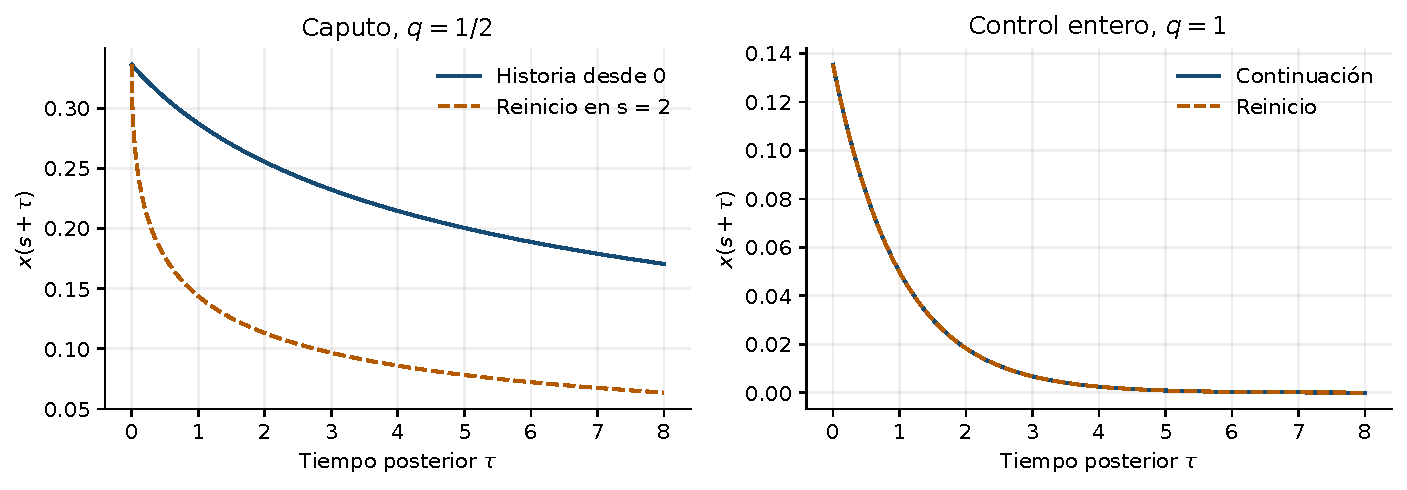
\includegraphics[width=.96\linewidth]{figures/revision/reinicio_caputo.pdf}
\caption{Soluciones analíticas de $D^q x=-x$, con $x(0)=1$ y reinicio en
$s=2$. En $q=1/2$ se usa la identidad~\eqref{eq:rev-mittag-half}; en $q=1$
se usa la exponencial. La coincidencia del valor de arranque no conserva la
evolución fraccionaria. Las curvas se evalúan a partir de sus soluciones analíticas.}
\label{fig:rev-reinicio}
\end{hafocommonfigure}

Este ejemplo complementa el contraste entre la respuesta estacionaria de
Weyl y la respuesta causal de Caputo del oscilador lineal forzado estudiado
por Duan, Lan y Li~\cite{DuanLanLi2022WeylCaputo}. Ese trabajo proporciona un
ejemplo analítico con transitorios de cola algebraica; no demuestra
persistencia de una órbita no lineal autónoma obtenida por balance armónico.

\subsection{Identidades algebraicas y clasificación local}

La transferencia y el espectro local se obtienen a partir del mismo campo.
Las identidades de la resolvente, del jacobiano y del determinante permiten
comprobar la coherencia entre ambas construcciones antes de integrar las
semillas.

Para la convención $b=(-\alpha,0,0)^{\mathsf T}$ y
$G(\lambda)=r^{\mathsf T}(\lambda I-P)^{-1}b$, el cierre es
$1-G((i\omega)^q)N=0$. Si se cambia la resolvente a
$(P-\lambda I)^{-1}$, se cambia simultáneamente el signo de la transferencia
y del cierre. Mezclar el signo de una convención con la resolvente de la otra
altera la semilla. El determinante y la identidad de realimentación se
comprobaron antes de evaluar ganancias.

En los parámetros nominales de Chua PWL, el margen de Matignon del origen
para $q=0.9998$ es aproximadamente $0.001486316766$ rad. En c590, el margen
de los equilibrios exteriores para $q=0.9999$ es $0.000742265117$ rad.
Estos cálculos apoyan la clasificación lineal local expuesta; no aportan un
radio de atracción certificado ni un margen frente a cualquier redondeo de
parámetros. Las hipótesis no lineales y la regularidad por regiones siguen
siendo necesarias.

En c590, el punto perpetuo de coordenada $x>0$ es aproximadamente
\[
 (1.213090022614,-20.187269924095,-21.549363340657).
\]
El producto $DF\,F$ se anula a la precisión declarada, mientras
$\|F\|\simeq545.09983035$. Esto comprueba la condición algebraica de PP,
pero también muestra que una raíz puede estar lejos de la respuesta de
interés y tener una velocidad inicial grande. La condición PP no contiene
por sí sola una prueba de captura, acotación o superioridad de la semilla.

Para Kalman--Fitts se recuperan los menores de Routh
$12.12174$ y $1.456324405056$, ambos positivos, y la ganancia directa
$k\simeq-0.043168701157$. El rango positivo de la función descriptiva de
$\tanh$ no contiene esa ganancia. El rechazo de la ruta directa es, por
tanto, un resultado informativo; cambiar de ruta debe conservar la
explicación de la obstrucción.

La comprobación de los pesos ABM produce residuos simbólicos nulos. No
identifica automáticamente dos implementaciones: el tratamiento del arranque,
el orden de suma, la precisión, la evaluación PECE y el transporte de historia
todavía pueden diferir. El límite $q=1$ recupera cuadraturas compuestas;
el predictor global no es, en general, el paso local de Euler iniciado en el
estado corregido. Para $\dot x=x$, la diferencia del segundo predictor es
$-h^2/2$, como se dedujo en la sección de integración.

\subsection{Comparación de respuestas y sensibilidad numérica}

En los casos enteros, el retorno cilíndrico de PLL y el ciclo de
Kalman--Fitts permiten comparar períodos y observables entre métodos.
La comparación Python--Julia de PLL y MAVPD coincide en 96 y 112
decisiones de destino, respectivamente. En los casos fraccionarios,
el reinicio autónomo PWL y las distintas implementaciones de c590
permiten examinar la influencia de la convolución y del horizonte.

En C02, la frecuencia dominante del control se reproduce, pero la máxima
diferencia de entropía espectral es $2.2243710\times10^{-4}$. Una frecuencia
dominante consistente no distingue por sí sola oscilación regular, transitorio
largo y caos. En c590, el núcleo general alcanza el umbral de norma en
$t=266.5$ para $h=0.005$, mientras el núcleo histórico recompilado completa
$T=300$. Los controles con $h=0.01$ y $0.0025$ también completan el horizonte.
Esta secuencia no permite afirmar convergencia bajo refinamiento ni atribuir
la diferencia automáticamente a sensibilidad caótica. Cada trayectoria corresponde a un integrador y a una ventana
concretos; la coincidencia visual entre proyecciones no basta para
resolver esa diferencia de evolución.

La discrepancia exige comparar sobre el mismo PVI los
pesos iniciales, las tablas, el orden de acumulación, la aritmética y las
trayectorias antes de la separación; después, contrastar un tercer método
independiente con control de error. Un umbral de divergencia es una regla de
parada computacional. Su cruce no demuestra una explosión matemática en
tiempo finito, y completar $T$ no demuestra acotación para todo tiempo.

\subsection{Muestreo finito y una cota que exige hipótesis adicionales}

Fijados un candidato de referencia, un integrador, una regla de clasificación
y una distribución $\mu$ sobre una región $R$, sea $p$ la probabilidad de
\emph{contacto clasificado} con ese candidato. El calificativo es esencial:
$p$ depende del protocolo y no es todavía la medida de una cuenca exacta.

\begin{proposition}[cero contactos bajo muestreo independiente]
Si $X_1,\ldots,X_n$ son muestras independientes con la misma distribución
$\mu$, la regla de clasificación permanece fija y cada muestra tiene
probabilidad $p$ de contacto, entonces la probabilidad de observar cero
contactos es $(1-p)^n$. Para un nivel $1-\delta$, la cota superior unilateral
que corresponde a observar cero es
\begin{equation}
 p_U=1-\delta^{1/n},\qquad 0<\delta<1.
 \label{eq:rev-binomial-zero}
\end{equation}
\end{proposition}
\begin{proof}
La independencia permite multiplicar las probabilidades $1-p$ de los $n$
no contactos. La función $(1-p)^n$ es decreciente en $p$. Como \(0<\delta<1\) y \(0\leq p_U<1\), podemos tomar
logaritmos:
\[
 (1-p_U)^n=\delta
 \ \Longrightarrow\ n\log(1-p_U)=\log\delta
 \ \Longrightarrow\ 1-p_U=e^{\log\delta/n}=\delta^{1/n}.
\]
Despejar \(p_U\) da \cref{eq:rev-binomial-zero}. Si \(p>p_U\),
entonces \(1-p<1-p_U\), y elevar a \(n>0\) conserva la desigualdad:
\(\Pr_p(0)=(1-p)^n<\delta\). La cota resulta de invertir este
contraste unilateral; no asigna una probabilidad posterior al parámetro.
\end{proof}

Con $1-\delta=0.95$, los tamaños $n=7200$ y $8400$ darían
$p_U\simeq0.0004159874$ y $0.0003565712$. Para \(n\) grande, la expansión de la exponencial permite ver su
dependencia con el tamaño de muestra:
\[
 p_U=1-e^{\log\delta/n}
 =-\frac{\log\delta}{n}
  -\frac{(\log\delta)^2}{2n^2}+O(n^{-3}).
\]
Estos valores corresponden a la hipótesis i.i.d. Las direcciones de una
malla esférica determinista no satisfacen esa hipótesis. Agrupar muestras
con cuotas fijas por radio tampoco las vuelve idénticamente distribuidas;
una mezcla aleatoria predefinida constituiría otro diseño. Por ello la cota no es un
intervalo de confianza para los sondeos deterministas de Chua. Además, una esfera no muestrea el volumen de toda la bola;
cambiar $R$ o $\mu$ cambia la cantidad que se estima.

\begin{hafocommonfigure}[htbp]
\centering
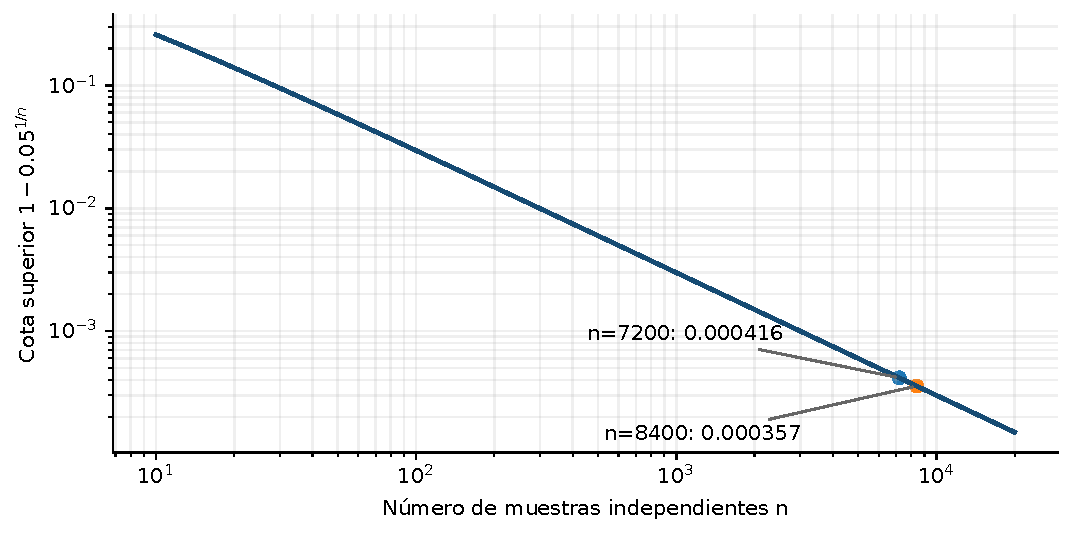
\includegraphics[width=.78\linewidth]{figures/revision/cota_iid_cero_contactos.pdf}
\caption{Cota matemática unilateral de contacto clasificado al observar
cero éxitos, condicionada a muestras i.i.d., clasificador fijo y nivel del
95\%. Los dos tamaños señalados ilustran la fórmula; no son una
certificación estadística de las campañas de malla determinista.}
\label{fig:rev-cota-iid}
\end{hafocommonfigure}

Aun cuando las hipótesis estadísticas se cumplan, $p_U>0$ para todo $n$
finito. La cota no demuestra que una vecindad completa esté separada de la
cuenca. Para esa conclusión se necesita un argumento local de estabilidad,
una inclusión validada u otro certificado que cubra todos sus puntos.

\subsection{Diseño de un contraste comparable entre rutas}

La comparación propuesta debe fijar primero un conjunto de sistemas y
parámetros que no se seleccione después de observar el éxito. Se compararán
la ruta Lur'e admisible, PP/FPP--A, semillas geométricas y una referencia
aleatoria o de malla. Si una ruta no es aplicable, su resultado es
\emph{no aplicable con causa demostrada}; no debe contarse como fallo de
integración ni omitirse del balance de cobertura.

Para cada sistema se fijarán el presupuesto de semillas, los recursos de
integración y los criterios de parada. La misma lista de campos, órdenes,
horizontes, escalas y políticas de memoria debe regir todas las rutas.
En Caputo se distinguirán dos experimentos: comparar reinicios sobre datos
constantes, o comparar historias transportadas dentro de un espacio
admisible. No es válido dar a una ruta una historia larga y a otra sólo un
estado puntual y atribuir la diferencia exclusivamente al generador.

La referencia de clasificación debe calibrarse con ventanas distintas de
las empleadas para validar las semillas. Se fijarán de antemano la distancia,
las coordenadas periódicas y los umbrales. El presupuesto debe informar
evaluaciones del campo, pasos e historia procesada; el número de semillas
por sí solo no iguala costos entre un flujo entero y una convolución de
memoria completa. Los tiempos de máquina son medidas descriptivas, no una
propiedad matemática del método.

Los desenlaces mínimos serán: fracción de semillas admisibles; fracción que
supera controles de integración; número de respuestas distintas bajo la
regla declarada; costo hasta el primer candidato; estabilidad de la decisión
frente a paso y horizonte; y contactos clasificados por equilibrio y radio.
Los fallos numéricos deben conservar una categoría propia. El conjunto de
configuraciones sin resultado se contabiliza por separado, pues excluirlas
sesgaría la comparación hacia los casos favorables.

Un experimento de ablación retirará por separado el filtro de realizabilidad,
la continuidad de historia y el filtro geométrico. Ese diseño permite
preguntar qué aporta cada componente. Las hipótesis que se contrastarán son
una mejora de rendimiento \emph{bajo el protocolo}, su costo y su cobertura,
no la existencia universal de atractores ocultos. El piloto registrado
constituye una prueba de viabilidad; sus tamaños, contratos y selecciones no
reemplazan esta comparación prospectiva.

\subsection{Antecedentes recientes que delimitan la propuesta}

Doan y Kloeden~\cite{DoanKloeden2022Triangular} prueban resultados para una
clase triangular de producto, con hipótesis de disipación y no degeneración.
La estructura triangular por sí sola no basta y esos resultados no se
trasladan automáticamente a un sistema general de Chua, Lorenz o RF. En el
marco funcional reciente de Cui, Kloeden y Xin
\cite{CuiKloedenXin2026CaputoDynamics}, el resultado de existencia citado es
precompacto en su universo declarado; la compactitud genérica queda abierta.
La proyección a valores actuales tampoco identifica por sí sola una cuenca
funcional. Estas distinciones afectan la formulación del objetivo, no sólo
la terminología.

Los trabajos de Danca y Fečkan y de Danca
\cite{DancaFeckan2024MemoryPrinciple,Danca2026ImprovedLyapunov} son pertinentes
para discutir algoritmos de exponentes. En ellos debe leerse la expresión
\emph{memoria completa} junto con el esquema impulsivo y el cambio del
terminal inferior de cada segmento. Esa denominación no demuestra
conservación del PVI causal original durante una renormalización QR.
Un método distinto puede ser útil, pero deben identificarse el sistema
variacional, las operaciones sobre su historia y el objeto que estima.

La validación de bloques aislantes para flujos de Stephens y Wanner
\cite{StephensWanner2014IsolatingBlocks} y el análisis numérico riguroso
infinito dimensional de Day, Junge y Mischaikow
\cite{DayJungeMischaikow2004InfiniteDimensional} orientan una posible etapa
de certificación. Se citan como antecedentes de herramientas y requisitos;
no como pruebas ya implementadas en estas campañas. Una discretización de
memoria necesita cotas de error y una transferencia rigurosa al sistema
original antes de heredar un índice topológico.

Finalmente, la aproximación de núcleos por sumas de exponenciales
\cite{JiangZhangZhangZhang2017FastCaputo} puede comprimir contribuciones de
toda la historia dentro de un intervalo y una tolerancia declarados. Es
distinta de borrar una cola. Las cotas obtenidas para problemas de difusión
no certifican automáticamente el seguimiento prolongado de una trayectoria
no lineal sensible ni sus invariantes dinámicos. Su uso exige una estimación
de error propia, además de una comparación de costo.

\subsection{Alcance de la comparación}

La eficacia de un generador de semillas depende del sistema, del destino
buscado y de los recursos que exige integrar cada condición. Los resultados
de PLL y MAVPD permiten medir cobertura y costo dentro de sus dominios;
la generalización requiere otras configuraciones. En Caputo, además,
la comparación debe conservar la misma clase de historias para atribuir
una diferencia al generador.

El contraste de c590 identifica una sensibilidad concreta que afecta a
la clasificación de cuencas. Los métodos de grado y los bloques aislantes
ofrecen una vía para complementar el muestreo con argumentos que cubran
regiones completas. En un sistema con memoria, esa vía exige también
controlar el error de la aproximación del operador y su relación con
el espacio funcional original.

\ifHAFOPedagogy
\begin{bloqueestudio}{Ejercicios}
\begin{enumerate}
 \item Derive~\eqref{eq:rev-binomial-zero} y explique por qué no se aplica a
 una malla determinista. Distinga contacto clasificado y pertenencia a una
 cuenca exacta. Compruebe que $p_U$ es positivo para todo $n$ finito.
 \item Compare el arranque tras $s>0$ del ejemplo lineal fraccionario.
 Identifique qué hipótesis permite usar $O(\tau)$ en la continuación y
 $\tau^q$ en el reinicio. Repita el razonamiento para $q=1$.
 \item Escriba una tabla de cuatro rutas para un sistema elegido. Declare
 las no aplicables, el presupuesto común y un control negativo. Explique cómo cambia el costo al aumentar el horizonte de memoria.
 \item Compare las decisiones de destino de c590 al cambiar método y paso.
 Explique por qué completar un horizonte y cruzar una norma umbral son
 observaciones distintas de la acotación matemática para todo tiempo.
\end{enumerate}
\end{bloqueestudio}
\fi
